\documentclass[10pt,a4paper,twocolumn]{article}

\usepackage[a4paper,margin=2cm]{geometry}
\usepackage{amsmath}
\usepackage{booktabs}
\usepackage{graphicx}
\usepackage{hyperref}
\usepackage{graphicx}
\usepackage{float}

\title{Machine Learning Project 1}
\author{Marco Valerio Marmo, Giovanni Nostro, Isaia Mossi \\ EPFL}
\date{}
\begin{document}
\maketitle

\section{Introduction}

Cardiovascular diseases are among the leading causes of death worldwide.
The goal of this project is to predict the presence of myocardial infarction or coronary heart disease (MICHD) from lifestyle and clinical variables contained in the BRFSS dataset.

The dataset contains more than 300,000 samples and several hundred health-related features describing demographics, medical conditions and behavioral habits.
The task is formulated as a binary classification problem.

\section{Exploratory Data Analysis}

The dataset contains 321 original features describing demographic, clinical and lifestyle information collected through the BRFSS survey.
A train-validation split (80\%-20\%) was performed using a fixed random seed in order to evaluate model performance.

An initial analysis revealed that the dataset is highly imbalanced, with only approximately 8.8\% of individuals belonging to the positive class.
Because of this imbalance, accuracy alone is not an appropriate evaluation metric and the F1-score was used throughout the project.

\begin{figure}[H]
    \centering
    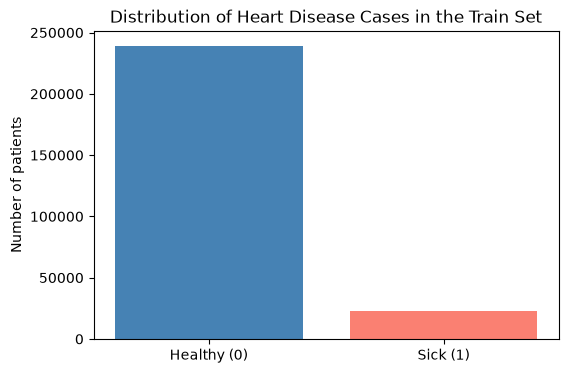
\includegraphics[width=0.8\linewidth]{images/disease_cases.png}
    \caption{Distribution of healthy and diseased patients in the training set. The dataset is strongly imbalanced, with only about 8.8\% positive samples.}
    \label{fig:classdist}
\end{figure}

Figure~\ref{fig:classdist} highlights the severe class imbalance present in the dataset.
Consequently, the learning algorithms must be able to identify a relatively small number of positive cases among a large majority of healthy individuals.

To better understand the dataset, we investigated the relationship between cardiovascular disease and known risk factors.
Age and sex are widely recognized predictors of cardiovascular risk and were therefore examined during the exploratory analysis.

\begin{figure}[H]
    \centering
    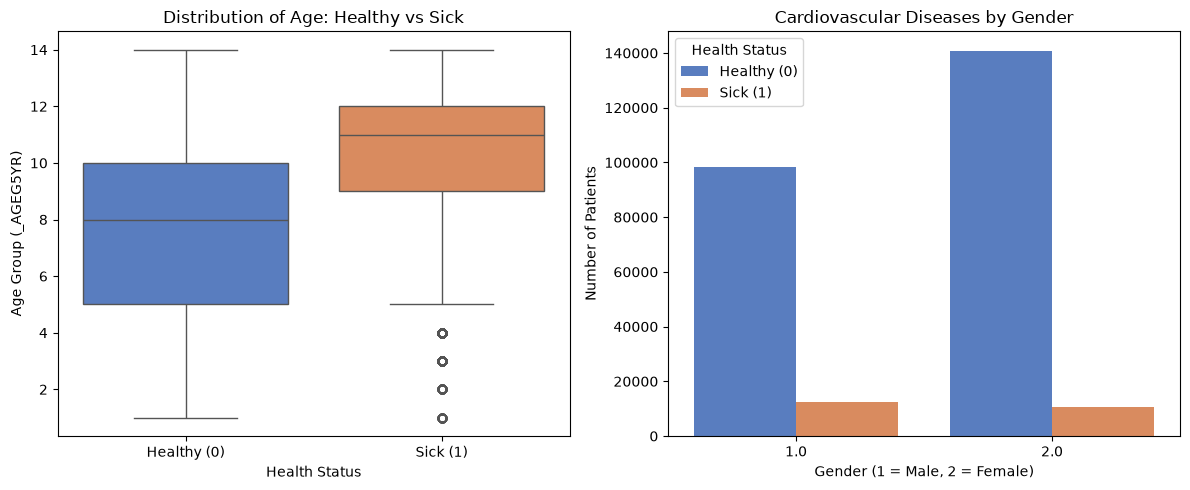
\includegraphics[width=1\linewidth]{images/age_and_gender_distribution.png}
    \caption{Relationship between cardiovascular disease, age and gender. Older age groups exhibit a substantially higher disease prevalence.}
    \label{fig:agegender}
\end{figure}

As shown in Figure~\ref{fig:agegender}, cardiovascular disease becomes more prevalent in older age groups.
This observation is consistent with established medical knowledge and provides evidence that the dataset contains meaningful predictive information.

\section{Data Preprocessing}

The large number of categorical features required extensive preprocessing.

Categorical variables were transformed using one-hot encoding in order to obtain a suitable representation for linear models. Missing values in numerical features were replaced by the median value computed on the training set.
After imputation, numerical variables were standardized to zero mean and unit variance. Finally, an intercept term was added to all samples.

Because one-hot encoding considerably increased the dimensionality of the data, additional feature selection was performed before training the final models.

\section{Feature Selection}

After one-hot encoding, the number of features increased substantially, resulting in a very high-dimensional representation of the dataset.
Furthermore, a correlation analysis revealed the presence of numerous highly correlated variables, indicating a significant amount of redundant information.

To reduce dimensionality and improve computational efficiency, we performed feature selection using an L1-regularized logistic regression model.
The sparsity-inducing L1 penalty drives many coefficients toward zero, making it possible to identify the most informative variables.

The objective of this step was not to maximize predictive performance but rather to construct a compact subset of features for subsequent models.
Features associated with near-zero coefficients were discarded, while the remaining variables were retained.

This procedure reduced the feature space to approximately 418 selected features, including the intercept term.
The resulting representation was used for all subsequent classification experiments.

\section{Models}

Our modelling strategy followed an iterative approach.

As an initial baseline, we implemented a linear Support Vector Machine (SVM).
The objective was to assess whether a linear classifier could extract useful information from the high-dimensional feature space obtained after preprocessing.

The severe class imbalance of the dataset motivated the use of logistic regression, which provides probabilistic outputs and allows the decision threshold to be optimized according to the evaluation metric.

Feature selection was performed through L1-regularized logistic regression.
The selected features were subsequently used to train a standard logistic regression model.

Finally, we investigated a weighted logistic regression approach, where larger weights were assigned to positive samples in order to compensate for the low prevalence of cardiovascular disease cases.

\section{Results}

The primary challenge of this project was the strong class imbalance of the dataset, with positive samples representing less than 10\% of the observations.
This characteristic had a significant impact on model selection and performance.

The initial linear SVM baseline struggled to correctly identify positive cases and tended to favor the majority class. We therefore shifted our focus to probabilistic models based on logistic regression.

After applying one-hot encoding, median imputation, feature standardization and L1-based feature selection, logistic regression achieved the best overall performance.
The decision threshold was tuned on the validation set using the F1-score, which was considered more appropriate than accuracy due to the class imbalance.

To further address the imbalance issue, we implemented a weighted logistic regression assigning larger weights to positive samples during training.
While this modification increased the influence of minority examples, it did not translate into an improvement in validation performance.

Table~\ref{tab:results} summarizes the final results obtained by the different approaches.

\begin{table}[t]
    \centering
    \begin{tabular}{lc}
        \toprule
        Model & Validation F1-score \\
        \midrule
        Logistic Regression & 0.432 \\
        Weighted Logistic Regression & 0.424 \\
        Linear SVM & 0.358 \\
        \bottomrule
    \end{tabular}
    \caption{Validation performance of the evaluated models.}
    \label{tab:results}
\end{table}

\section{Conclusions}

Standard logistic regression achieved the highest validation F1-score, outperforming both the weighted version and the linear SVM.
These results suggest that the improvements provided by preprocessing and feature selection were more important than additional class reweighting.
Consequently, logistic regression was selected as the final model for the generation of test predictions.

\end{document}